%%%%%%%%%%%%%%%%%%%%%%%%%%%%%%%%%%%%%%%%%%%%%%%%%%%%%%%%%%%%%%%
%% OXFORD THESIS TEMPLATE

% Use this template to produce a standard thesis that meets the Oxford University requirements for DPhil submission
%
% Originally by Keith A. Gillow (gillow@maths.ox.ac.uk), 1997
% Modified by Sam Evans (sam@samuelevansresearch.org), 2007
% Modified by John McManigle (john@oxfordechoes.com), 2015
% Modified by Ulrik Lyngs (ulrik.lyngs@cs.ox.ac.uk), 2018, for use with R Markdown
%
% Ulrik Lyngs, 25 Nov 2018: Following John McManigle, broad permissions are granted to use, modify, and distribute this software
% as specified in the MIT License included in this distribution's LICENSE file.
%
% John tried to comment this file extensively, so read through it to see how to use the various options.  Remember
% that in LaTeX, any line starting with a % is NOT executed.  Several places below, you have a choice of which line to use
% out of multiple options (eg draft vs final, for PDF vs for binding, etc.)  When you pick one, add a % to the beginning of
% the lines you don't want.


%%%%% CHOOSE PAGE LAYOUT
% The most common choices should be below.  You can also do other things, like replacing "a4paper" with "letterpaper", etc.

% This one will format for two-sided binding (ie left and right pages have mirror margins; blank pages inserted where needed):
%\documentclass[a4paper,twoside]{templates/ociamthesis}
% This one will format for one-sided binding (ie left margin > right margin; no extra blank pages):
%\documentclass[a4paper]{ociamthesis}
% This one will format for PDF output (ie equal margins, no extra blank pages):
%\documentclass[a4paper,nobind]{templates/ociamthesis}
%UL 2 Dec 2018: pass this in from YAML
\documentclass[a4paper, nobind]{templates/ociamthesis}


% UL 30 Nov 2018 pandoc puts lists in 'tightlist' command when no space between bullet points in Rmd file
\providecommand{\tightlist}{%
  \setlength{\itemsep}{0pt}\setlength{\parskip}{0pt}}
 
% UL 1 Dec 2018, fix to include code in shaded environments

%UL 2 Dec 2018 reduce whitespace around verbatim environments
\usepackage{etoolbox}
\makeatletter
\preto{\@verbatim}{\topsep=0pt \partopsep=0pt }
\makeatother

%UL 26 Mar 2019, enable strikethrough
\usepackage[normalem]{ulem}

%UL 15 Oct 2019, enable link highlighting to be turned off from YAML
\usepackage[colorlinks=false,pdfpagelabels,hidelinks=true]{hyperref}

%%%%% SELECT YOUR DRAFT OPTIONS
% Three options going on here; use in any combination.  But remember to turn the first two off before
% generating a PDF to send to the printer!

% This adds a "DRAFT" footer to every normal page.  (The first page of each chapter is not a "normal" page.)

% This highlights (in blue) corrections marked with (for words) \mccorrect{blah} or (for whole
% paragraphs) \begin{mccorrection} . . . \end{mccorrection}.  This can be useful for sending a PDF of
% your corrected thesis to your examiners for review.  Turn it off, and the blue disappears.
\correctionstrue

%%%%% BIBLIOGRAPHY SETUP
% Note that your bibliography will require some tweaking depending on your department, preferred format, etc.
% The options included below are just very basic "sciencey" and "humanitiesey" options to get started.
% If you've not used LaTeX before, I recommend reading a little about biblatex/biber and getting started with it.
% If you're already a LaTeX pro and are used to natbib or something, modify as necessary.
% Either way, you'll have to choose and configure an appropriate bibliography format...

% The science-type option: numerical in-text citation with references in order of appearance.
% \usepackage[style=numeric-comp, sorting=none, backend=biber, doi=false, isbn=false]{biblatex}
% \newcommand*{\bibtitle}{References}

% The humanities-type option: author-year in-text citation with an alphabetical works cited.
% \usepackage[style=authoryear, sorting=nyt, backend=biber, maxcitenames=2, useprefix, doi=false, isbn=false]{biblatex}
% \newcommand*{\bibtitle}{Works Cited}

%UL 3 Dec 2018: set this from YAML in index.Rmd
\usepackage[style=authoryear, sorting=nyt, backend=biber, maxcitenames=2, useprefix, doi=true, isbn=false, uniquename=false]{biblatex}
\newcommand*{\bibtitle}{Works Cited}

% This makes the bibliography left-aligned (not 'justified') and slightly smaller font.
\renewcommand*{\bibfont}{\raggedright\small}

% Change this to the name of your .bib file (usually exported from a citation manager like Zotero or EndNote).
\addbibresource{references.bib}


% Uncomment this if you want equation numbers per section (2.3.12), instead of per chapter (2.18):
%\numberwithin{equation}{subsection}


%%%%% THESIS / TITLE PAGE INFORMATION
% Everybody needs to complete the following:
\title{Determining the Influence of Different Variables on the Price of Ikea Products\\
-- a Regression Analysis}
\author{Philip Krück, Johannes Pein}
\college{}

% Master's candidates who require the alternate title page (with candidate number and word count)
% must also un-comment and complete the following three lines:
%\masterssubmissiontrue
%\candidateno{933516}
%\wordcount{28,815}

% Uncomment the following line if your degree also includes exams (eg most masters):
%\renewcommand{\submittedtext}{Submitted in partial completion of the}
% Your full degree name.  (But remember that DPhils aren't "in" anything.  They're just DPhils.)
\degree{B.Sc. Business Informatics (A Track)}
% Term and year of submission, or date if your board requires (eg most masters)
\degreedate{04.12.2020}


%%%%% YOUR OWN PERSONAL MACROS
% This is a good place to dump your own LaTeX macros as they come up.
\modulename{Digital Toolbox: Data Business}
\lecturer{Lecturer: Ulf Köther}
\groupnumber{Group Number: 7}
\matriculationnumbers{Matriculation Numbers: 3938 (P.Krück), **** (J.Pein)}


% To make text superscripts shortcuts
	\renewcommand{\th}{\textsuperscript{th}} % ex: I won 4\th place
	\newcommand{\nd}{\textsuperscript{nd}}
	\renewcommand{\st}{\textsuperscript{st}}
	\newcommand{\rd}{\textsuperscript{rd}}

%%%%% THE ACTUAL DOCUMENT STARTS HERE
\begin{document}

%%%%% CHOOSE YOUR LINE SPACING HERE
% This is the official option.  Use it for your submission copy and library copy:
\setlength{\textbaselineskip}{22pt plus2pt}
% This is closer spacing (about 1.5-spaced) that you might prefer for your personal copies:
%\setlength{\textbaselineskip}{18pt plus2pt minus1pt}

% You can set the spacing here for the roman-numbered pages (acknowledgements, table of contents, etc.)
\setlength{\frontmatterbaselineskip}{17pt plus1pt minus1pt}


% UL: You can set the general paragraph spacing here - I've set it to 2pt (was 0) so
% it's less claustrophobic
\setlength{\parskip}{2pt plus 1pt}


% Leave this line alone; it gets things started for the real document.
\setlength{\baselineskip}{\textbaselineskip}


%%%%% CHOOSE YOUR SECTION NUMBERING DEPTH HERE
% You have two choices.  First, how far down are sections numbered?  (Below that, they're named but
% don't get numbers.)  Second, what level of section appears in the table of contents?  These don't have
% to match: you can have numbered sections that don't show up in the ToC, or unnumbered sections that
% do.  Throughout, 0 = chapter; 1 = section; 2 = subsection; 3 = subsubsection, 4 = paragraph...

% The level that gets a number:
\setcounter{secnumdepth}{2}
% The level that shows up in the ToC:
\setcounter{tocdepth}{2}


% JEM: Pages are roman numbered from here, though page numbers are invisible until ToC.  This is in
% keeping with most typesetting conventions.
\begin{romanpages}

% Title page is created here
\maketitle

%%%%% MINI TABLES
% This lays the groundwork for per-chapter, mini tables of contents.  Comment the following line
% (and remove \minitoc from the chapter files) if you don't want this.  Un-comment either of the
% next two lines if you want a per-chapter list of figures or tables.
  \dominitoc % include a mini table of contents

% This aligns the bottom of the text of each page.  It generally makes things look better.
\flushbottom

% This is where the whole-document ToC appears:
\tableofcontents

%%%%% LIST OF ABBREVIATIONS
% This example includes a list of abbreviations.  Look at text/abbreviations.tex to see how that file is
% formatted.  The template can handle any kind of list though, so this might be a good place for a
% glossary, etc.
% First parameter can be changed eg to "Glossary" or something.
% Second parameter is the max length of bold terms.
\begin{mclistof}{List of Abbreviations}{3.2cm}

\item[R] Statistical Programming Language
\item[MSE] Mean Squared Error
\item[IQR] Interquartile Range

\end{mclistof} 


% The Roman pages, like the Roman Empire, must come to its inevitable close.
\end{romanpages}

%%%%% CHAPTERS
% Add or remove any chapters you'd like here, by file name (excluding '.tex'):
\flushbottom

% all your chapters and appendices will appear here
\hypertarget{intro}{%
\chapter{Introduction}\label{intro}}

\begin{figure}
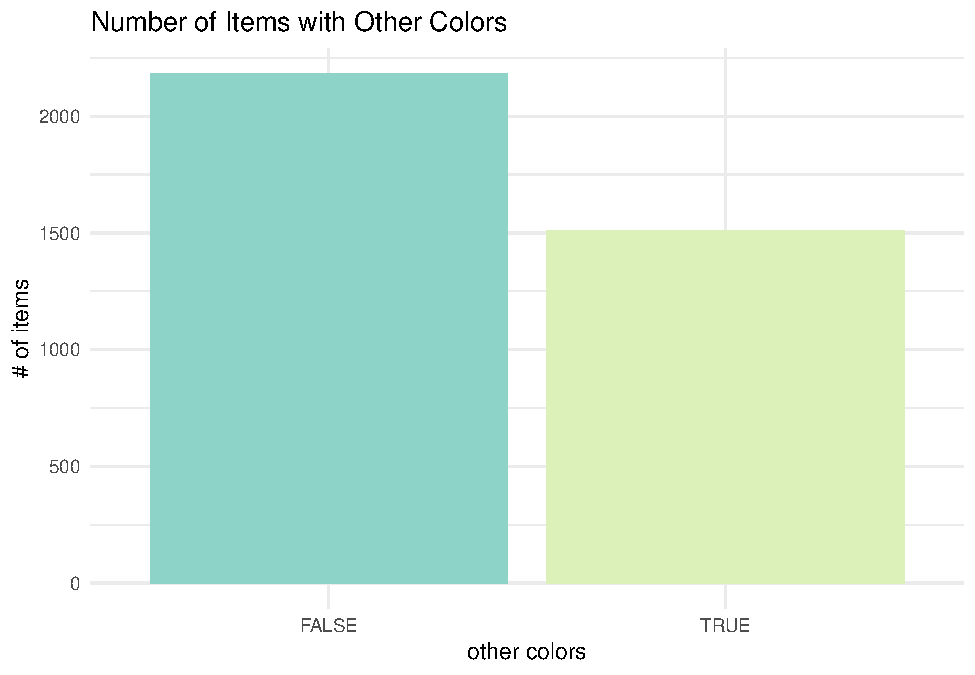
\includegraphics[width=1\linewidth]{_main_files/figure-latex/unnamed-chunk-3-1} \caption{Sample plot}\label{fig:unnamed-chunk-3}
\end{figure}

\hypertarget{theoretical-background-research-question}{%
\chapter{Theoretical Background \& Research Question}\label{theoretical-background-research-question}}

\hypertarget{theoretical_background}{%
\section{Theoretical Background}\label{theoretical_background}}

\hypertarget{data-set}{%
\subsection{Data Set}\label{data-set}}

The data set was obtained by a kaggle.com user (Reem Abdulrahman) by the means of webscraping techniques from the Saudi Arabian Ikea website in the furniture category on the 20th of April 2020. Noteworthy features include the name, category, price in Saudi Riyals, the designer and dimensions (width, height and depth). The data set has 13 variables and 2962 observations.

\hypertarget{overfitting}{%
\subsection{Overfitting}\label{overfitting}}

-\textgreater{}Johannes

\hypertarget{rf-basics}{%
\subsection{RF Basics}\label{rf-basics}}

-\textgreater{}Johannes

\hypertarget{feature-importance}{%
\subsection{Feature Importance}\label{feature-importance}}

-\textgreater{}Johannes

\hypertarget{research_question}{%
\section{Research Question}\label{research_question}}

This paper explores the influence for different variables on the price in the given data set. The motivating forces for this research question are the possible implications for price determination of new items.

\hypertarget{methods}{%
\chapter{Methods}\label{methods}}

\hypertarget{datacleaning}{%
\section{Data Cleaning and Transformatoin}\label{datacleaning}}

To examine the given data set properly, the authors first had to restructure and reformat it. This initial data cleaning step included type conversion, value mutation, addition of newly calculated fields and the removal of irrelevant columns.
Concretely, name, category and designer were converted to categorical variables. In the designer column, blank strings and values prefixed by ``IKEA of Sweden'' were converted to missing values (\texttt{NA}). Furthermore, both the price and old price were converted to double values and the currency was changed from Saudi Arabian Riyals to Euros based on the exchange rate from the time the data set was obtained by the author @ref(\#theoretical\_background).

Interestingly, the data set had a peculiarity where some rows were exact duplicates except for the category value. The authors considered multiple approaches to handle these data duplications without losing information about the category of an item.

One considered option was to merge the two category values into one column value via comma separation (e.g. \texttt{"a"} and \texttt{"b"} converts to \texttt{"a,\ b"}). However, this approach leads to the creation of many combinatorial categories with a low count of items per category which also reduces the item count per category where the category isn't comma separated. Overall this would lead to having many small categories which increases the difficulty in applying a regression model due to overfitting @ref(\#overfitting).

The second option was to create separate columns for the different values of \texttt{category}. The data set would then have observations with category one, two and three. While no information is lost utilizing this approach, most observations in the second and third category column would contain missing values, thus increasing the difficulty of analysis using a predefined model @\ref(\#random\_forest\_model).

The authors chose the option of selecting the observations out of the duplicates where the category count occurred most frequently when considering duplicates. The most important categories could be retained without including more column vectors into the data set as in option two.

To better facilitate the comparison of the different sizes of furniture items, the size in cubic meters was computed based on the depth, width and height values, and added as a column vector for further analysis.
Finally, the authors only selected columns that could have a potential impact on the analysis @ref(\#research\_question) for further investigation. A detailed comparison of the initial vs.~transformed data structure can be seen in tables \ref{tab:initial-ikea} and \ref{tab:tidy-ikea}.

TODO: Format these tables

\begin{table}

\caption{\label{tab:initial-ikea}Initial Data Set formatting.}
\centering
\begin{tabular}[t]{r|r|l|l|r|l|l|l|l|l|l|r|r|r}
\hline
X1 & item\_id & name & category & price & old\_price & sellable\_online & link & other\_colors & short\_description & designer & depth & height & width\\
\hline
0 & 90420332 & FREKVENS & Bar furniture & 2650 & No old price & TRUE & https://www.ikea.com/sa/en/p/frekvens-bar-table-in-outdoor-black-90420332/ & No & Bar table, in/outdoor,          51x51 cm & Nicholai Wiig Hansen & NA & 99 & 51\\
\hline
1 & 368814 & NORDVIKEN & Bar furniture & 9950 & No old price & FALSE & https://www.ikea.com/sa/en/p/nordviken-bar-table-black-00368814/ & No & Bar table,          140x80 cm & Francis Cayouette & NA & 105 & 80\\
\hline
2 & 9333523 & NORDVIKEN / NORDVIKEN & Bar furniture & 20950 & No old price & FALSE & https://www.ikea.com/sa/en/p/nordviken-nordviken-bar-table-and-4-bar-stools-black-black-s09333523/ & No & Bar table and 4 bar stools & Francis Cayouette & NA & NA & NA\\
\hline
3 & 80155205 & STIG & Bar furniture & 690 & No old price & TRUE & https://www.ikea.com/sa/en/p/stig-bar-stool-with-backrest-black-silver-colour-80155205/ & Yes & Bar stool with backrest,          74 cm & Henrik Preutz & 50 & 100 & 60\\
\hline
4 & 30180504 & NORBERG & Bar furniture & 2250 & No old price & TRUE & https://www.ikea.com/sa/en/p/norberg-wall-mounted-drop-leaf-table-white-30180504/ & No & Wall-mounted drop-leaf table,          74x60 cm & Marcus Arvonen & 60 & 43 & 74\\
\hline
5 & 10122647 & INGOLF & Bar furniture & 3450 & No old price & TRUE & https://www.ikea.com/sa/en/p/ingolf-bar-stool-with-backrest-white-10122647/ & No & Bar stool with backrest,          63 cm & Carina Bengs & 45 & 91 & 40\\
\hline
\end{tabular}
\end{table}

\begin{table}

\caption{\label{tab:tidy-ikea}Data Set after cleaning process.}
\centering
\begin{tabular}[t]{l|l|r|r|l|l|l|r}
\hline
name & category & price\_eur & old\_price\_eur & sellable\_online & other\_colors & designer & size\_m3\\
\hline
FREKVENS & Bar furniture & 65.02 & NA & TRUE & FALSE & Nicholai Wiig Hansen & NA\\
\hline
NORDVIKEN & Bar furniture & 244.14 & NA & FALSE & FALSE & Francis Cayouette & NA\\
\hline
NORDVIKEN / NORDVIKEN & Bar furniture & 514.05 & NA & FALSE & FALSE & Francis Cayouette & NA\\
\hline
STIG & Bar furniture & 16.93 & NA & TRUE & TRUE & Henrik Preutz & 0.30\\
\hline
NORBERG & Bar furniture & 55.21 & NA & TRUE & FALSE & Marcus Arvonen & 0.19\\
\hline
INGOLF & Bar furniture & 84.65 & NA & TRUE & FALSE & Carina Bengs & 0.16\\
\hline
\end{tabular}
\end{table}

\hypertarget{tbd}{%
\section{Exploratory Data Analysis}\label{tbd}}

The following sections explore our data based on the eight step data exploration protocol proposed by Zuur et al \autocite{Zuur2010}.

\hypertarget{step-1-outliers-in-price-and-independent-variables}{%
\subsection{Step 1: Outliers in Price and Independent Variables}\label{step-1-outliers-in-price-and-independent-variables}}

Outliers of the chosen variables (from tidying see @ref(\#datacleaning) can be observed for each variable (see plot \ldots{}).
The authors assume that outliers do not occur randomly in the form of an observer error. Web scraping code is written in a generic form which makes it generalizable to all applied pages. Thus takes human observation errors out of the equation. Additionally, the authors looked at individual outlier (stichprobenartig) examples and used the provided link column to manually double check observations against machine errors.
By the stated assumption, all outliers are meaningful for further analysis.

\hypertarget{step-2-homogeneity-of-price}{%
\subsection{Step 2: Homogeneity of Price}\label{step-2-homogeneity-of-price}}

The homogeneity (homoscedasticity) of variance for price is explored by the means of conditional boxplotting.
Within each name, and within each category the variance is heterogenous (\ref{fig:homogeneity}). However, looking at both name and category in conjunction, it is possible to explore homoscedasticity of variance for price.
In the context of this paper, the authors weren't able to inspect all variable combinations for the five categorical variables (\(2^3=8\)).

\begin{figure}
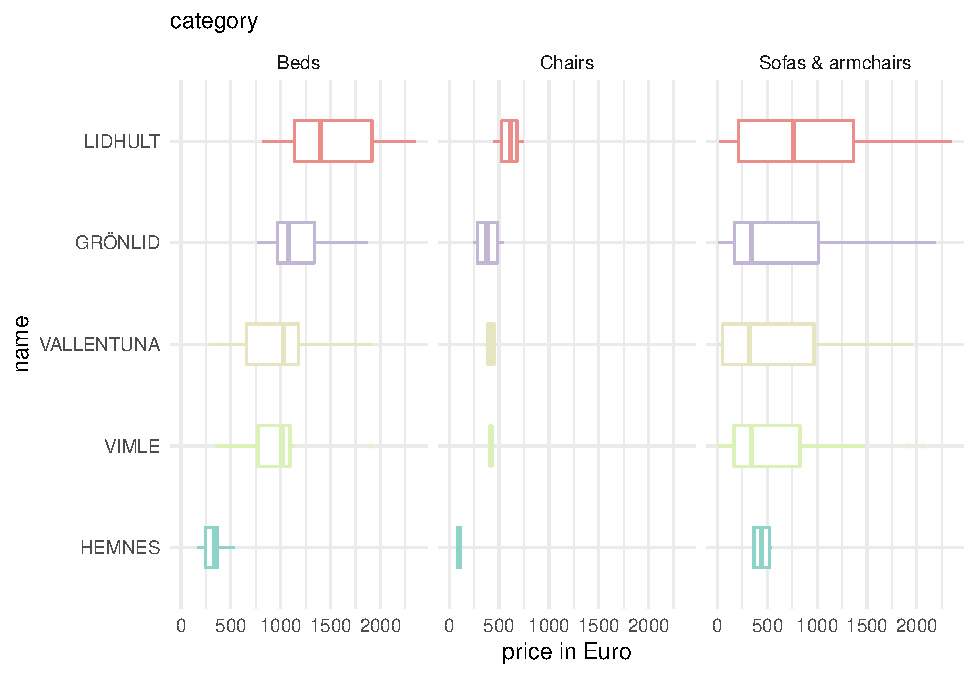
\includegraphics[width=1\linewidth]{_main_files/figure-latex/homogeneity-1} \caption{Homogeneity of category for selected combinations of name and category}\label{fig:homogeneity}
\end{figure}

\hypertarget{step-3-missing-value-trouble}{%
\subsection{Step 3: Missing Value Trouble}\label{step-3-missing-value-trouble}}

All numerical variables (\texttt{price}, \texttt{old\_price} and \texttt{size\_m3}) aren't arranged along a normal distribution (see \ref{fig:normality}), but rather follow an exponential decay (\(e^{-x}\)).

\begin{figure}
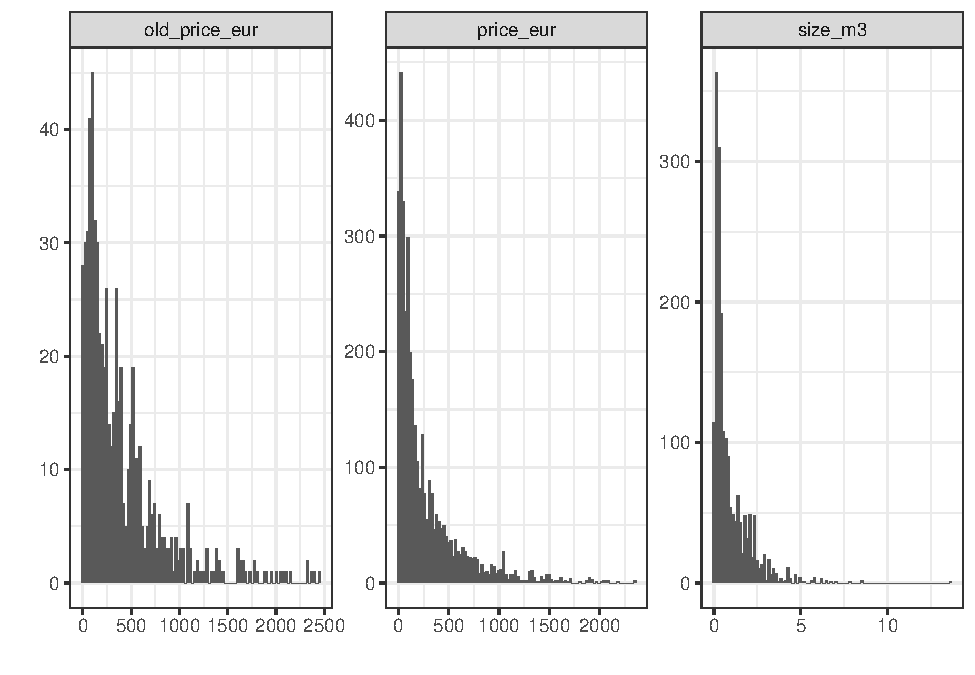
\includegraphics[width=1\linewidth]{_main_files/figure-latex/normality-1} \caption{Homogeneity of category for selected combinations of name and category}\label{fig:normality}
\end{figure}

\hypertarget{step-4-zeros}{%
\subsection{Step 4: Zeros}\label{step-4-zeros}}

\begin{itemize}
\tightlist
\item
  many missing values from old price -\textgreater{} assume those were not on sale
\item
  size\_m3 missing values because of calculation formula
\item
  designer -\textgreater{} removed values containing digits (were clearly falsely scraped)
\end{itemize}

\hypertarget{step-5-collinearity-between-independent-variables}{%
\subsection{Step 5: Collinearity between Independent Variables}\label{step-5-collinearity-between-independent-variables}}

\begin{itemize}
\tightlist
\item
  high collinearity between old price and price
\item
  relatively high collinearity between price and size
\item
  as can be seen in table
\end{itemize}

\hypertarget{step-6-relationship-between-independent-variables-and-price}{%
\subsection{Step 6: Relationship between Independent Variables and Price}\label{step-6-relationship-between-independent-variables-and-price}}

\begin{itemize}
\tightlist
\item
  from eda\_covariance.Rc (in Anhang + verweisen)
\item
  strong relationship b/w price + old price \& b/w price + size (see )
\item
  other relationships aren't strong
\end{itemize}

\hypertarget{step-7-interactions}{%
\subsection{Step 7: Interactions}\label{step-7-interactions}}

\begin{itemize}
\item
  Coplotting designer and name works, while the two combination would not plot
\item
  The linear model predicted infinite values and thus coplot the values properly for the other two options
\item
  However, dropping all NA values and thus reducing the total data size to 354 observations would case for the combination coplot name and category while name + designer combination would not work
\item
  The authors hypothesized that infinite values were caused by a division of zeros of the linear model since there occured 0 values in size
\item
  This however proved to be wrong after applying respective filters
\item
  The following interaction could be analyzed
\item
  \begin{itemize}
  \tightlist
  \item
    There is probably no significant interaction between size, price, name \& designer as can be seen in coplot -\textgreater{} lines are nearly parallel
  \end{itemize}
\item
  Based on the coplot of category and name with the 354 observations, inparallelity could be observed and thus could conclude a interaction. However, this could also be due to the small sample size
\item
\end{itemize}

(footnote): the authors would highly appreciate any solutions on this matter

\hypertarget{step-8-independence-of-price}{%
\subsection{Step 8: Independence of Price}\label{step-8-independence-of-price}}

\begin{itemize}
\tightlist
\item
  Durch das tidying in (cross reference) duplicate removal -\textgreater{} Zuur paper Step 8 1. citation: meaning that information from any one observation should not provide information on another after the effects of other variables have been accounted for. This concept is best explained with examples.
\end{itemize}

\hypertarget{random_forest_model}{%
\section{Random Forest Regression Model}\label{random_forest_model}}

\begin{itemize}
\tightlist
\item
  We chose rf
\item
  random forest erklären -\textgreater{} article (for in depth reference see article)
\item
  why random forest (not lm)? -\textgreater{} article to explain why random forest is great to explain feature importance

  \begin{itemize}
  \tightlist
  \item
    see article
  \item
    TODO: is normal distribution relevant for random forest (step 3) -\textgreater{} see article or site something
  \end{itemize}
\item
  To reproduce our results\ldots{} (\textcite{Johannes})

  \begin{itemize}
  \tightlist
  \item
    We chose randomForest R package for our analysis -\textgreater{} as in \ldots{} (cite article)
  \item
    data base is tidy ikea (step \ldots{})
  \item
    then transform this data set to apply rf (johannes)

    \begin{itemize}
    \tightlist
    \item
      remove old price because of high correlation factor (step 5 + 6) which would fuck up our overall result
    \item
      fct\_lump erklären
    \item
      rf has problems with na values -\textgreater{} 3 different methods to solve problem -\textgreater{} calculated 3 feature importances -\textgreater{} mean(a, b, c)
    \end{itemize}
  \end{itemize}
\end{itemize}

\hypertarget{results}{%
\chapter{Results}\label{results}}

\begin{itemize}
\tightlist
\item
  x-reference theoretical background: rf / variable importance
\item
  describe plot comprehensively -- w/ numbers from table
\end{itemize}

\hypertarget{discussion}{%
\chapter{Discussion}\label{discussion}}

\hypertarget{size_m3}{%
\section{size\_m3}\label{size_m3}}

\begin{itemize}
\tightlist
\item
  material cost
\item
  big items more expensive than small ones
\item
  high correlation to price
\end{itemize}

\hypertarget{designer}{%
\section{designer}\label{designer}}

\begin{itemize}
\item
  designers with high number of products produce products in wide price range : plot reference -\textgreater{} appendix
\item
  many different combinations of designer (49-53)
\item
  many designer-combinations with low number of products:

  \begin{itemize}
  \tightlist
  \item
    n combinations with occurrences\textless{}5
  \end{itemize}
\end{itemize}

-\textgreater{} overfitting: cite scholarly article
-\textgreater{} low generalization : model might perfom bad on other data

\hypertarget{name}{%
\section{name}\label{name}}

\begin{itemize}
\tightlist
\item
  overfitting
\end{itemize}

\hypertarget{category}{%
\section{category}\label{category}}

\begin{itemize}
\tightlist
\item
  beds are more expensive than chairs : some categories are more expensive than others (show plot)
\item
  but, price range varies heavily in category (show plot)
\end{itemize}

\hypertarget{other_colors}{%
\section{other\_colors}\label{other_colors}}

\begin{itemize}
\tightlist
\item
  products of every price range have both options : low importance
\item
  mean price is higher if other\_colors is true (show plot covariance price+other\_colors)
\item
  interquartile-range is smaller if other\_colors is false
\end{itemize}

\hypertarget{sellable_online}{%
\section{sellable\_online}\label{sellable_online}}

sellable true: price range too high
sellable ntrue: very rare

\hypertarget{conclusion-ausblick}{%
\section{Conclusion \& Ausblick}\label{conclusion-ausblick}}

\begin{itemize}
\tightlist
\item
  Further research:

  \begin{itemize}
  \tightlist
  \item
    analyze designer overfitting, recommend using overfitting techniques (e.g. \ldots{})
  \item
    analyze same research question with other techniques (lm, name more) and compare
  \item
    data scraping from other country-pages
  \end{itemize}
\end{itemize}

\hypertarget{individual-statements}{%
\chapter{Individual Statements}\label{individual-statements}}

\hypertarget{philip-kruxfcck}{%
\section{Philip Krück}\label{philip-kruxfcck}}

\hypertarget{johannes-pein}{%
\section{Johannes Pein}\label{johannes-pein}}

\startappendices

\hypertarget{plots}{%
\chapter{Plots}\label{plots}}

\hypertarget{plot-xyz}{%
\section{Plot xyz}\label{plot-xyz}}

\hypertarget{plot-abc}{%
\section{Plot abc}\label{plot-abc}}

\hypertarget{another-appendix}{%
\chapter{Another Appendix}\label{another-appendix}}


%%%%% REFERENCES

% JEM: Quote for the top of references (just like a chapter quote if you're using them).  Comment to skip.
% \begin{savequote}[8cm]
% The first kind of intellectual and artistic personality belongs to the hedgehogs, the second to the foxes \dots
%   \qauthor{--- Sir Isaiah Berlin \cite{berlin_hedgehog_2013}}
% \end{savequote}

\setlength{\baselineskip}{0pt} % JEM: Single-space References

{\renewcommand*\MakeUppercase[1]{#1}%
\printbibliography[heading=bibintoc,title={\bibtitle}]}

\end{document}
